
\chapter{Customization}
\label{cha:customization}

You you can customize Emacs in tree ways:
\begin{itemize}
\item using \keyword{Custom}, the interactive interface
\item using \keyword{Options} menu
\item adding lines of Lisp to you \argument{.emacs} file
\end{itemize}


No matter what method you use, though, the \argument{.emacs} startup file is modified.
Custom modifies it for you when you save settings through that interface.
The Options menu invokes Custom behind the scenes; when you choose Save Options, Custom again modifies \argument{.emacs}. 

\section{Using Options}
\label{sec:using-options}



\begin{figure}[!htp]
  \centering
  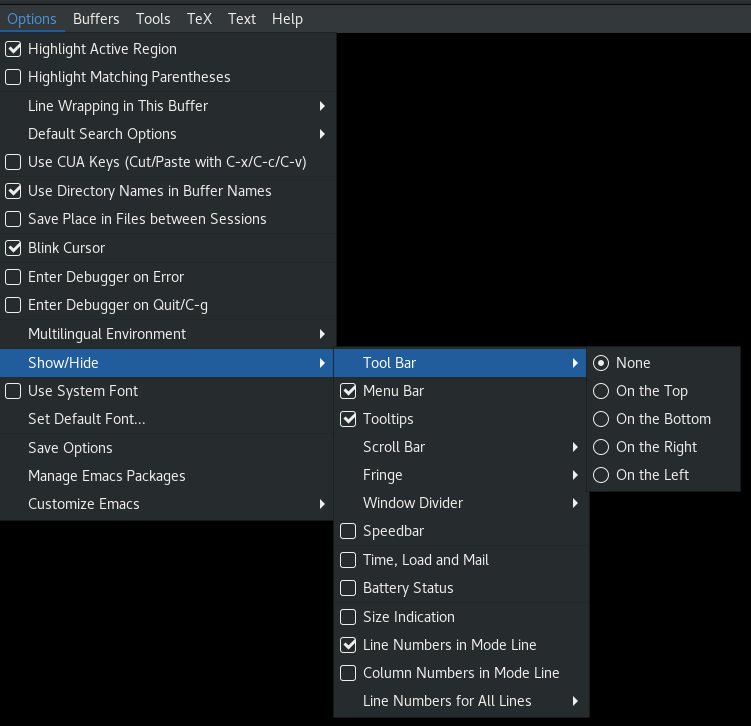
\includegraphics[width=0.6\textwidth]{hide-tool-bar}
  \caption{Using Options to hide toolbar}
  \label{fig:hide-tool-bar}
\end{figure}

Here the Figure \ref{fig:hide-tool-bar} to show how to use Options to hide toolbar.

\section{Using Custom}
\label{sec:using-custom}

Emacs now ships with a quirky graphical-but-not interface that allows you to customize most aspects of Emacs without knowing the gory details.
This feature, known as Custom, can be accessed by typing \keyword{M-x custom} or by clicking the tools icon on the toolbar.

\section{Modifying the .emacs File Directly}
\label{sec:modify-.emacs-file}

Emacs actually looks for a variety of startup files. In order, they are:
\begin{itemize}
\item \argument{.emacs.elc}: The byte-compiled Lisp version of your startup file. This is not editable, but can make startup quicker if you have a big, complex startup file.
\item \argument{.emacs.el}: The more formal name for your startup file. You can use Lisp commands to customize and initialize your entire Emacs environment.
\item \argument{.emacs}: The common name for the startup file. 
\item \argument{.emacs.d/init.el}
\end{itemize}

As soon as Emacs finds one of these files, that’s it; then it’s on to the next step in startup.


Here are some useful functions:
\begin{lstlisting}
;; This is the basic syntax.
(function-name arguments)
;; Example: Move forward one word.
(forward-word 1)

;; Set a value to a variable.
(setq variable-name variable-value)
;; Using setq-default has the advantage of setting the default value only.
;; Modes that choose to override this value may still do so.
(setq-default variable-name variable-value)
;; Example: set nil to indent-tabs-mode.
(setq-default indent-tabs-mode nil)

;; Add a hook to mode hook.
(add-hook 'hook-name 'hook-value)
;; Example: add font lock to emacs lisp mode
(add-hook 'emacs-lisp-mode-hook 'turn-on-font-lock)

;; Define key binding.
(define-key keymap "keystroke" 'command-name)
(global-set-key "keystroke" 'command-name)
(local-set-key "keystroke" 'command-name)
;; Example: bind goto-line to C-x l
(global-set-key "\C-xl" 'goto-line)
(define-key global-map "\C-xl" 'goto-line)
(define-key ctl-x-map "l" 'goto-line)

;; Unset key binding.
(global-unset-key "keystroke")
(define-key keymap "keystroke" nil)
;; Example: unset C-x l
(global-unset-key "C-xl")
(define-key clt-x-map "l" nil)
\end{lstlisting}

When define key binding,the three commands have the same effect but aren’t really any more efficient or better.
You can just use \argument{global-set-key} and use \argument{define-key} when setting the global key is not appropriate, such as when adding a mode-specific keystroke.
Here are some social characters for define key bindings shown in Table
\begin{table}[H]
  \centering
  \begin{tabular}{>{\textbackslash{}\bfseries}ll}
    \toprule
    \head{Special character} & \head{Meaning}\\
    \midrule
    C- & Control\\
    e & Esc\\
    M- & Meta\\
    n & Newline\\
    r & Enter\\
    t & Tab\\
    S- & shift\\
    H- & hyper\\
    s- & super\\
    A- & alt\\
    \bottomrule
  \end{tabular}
  \caption{Special characters}
  \label{tab:special-charaters}
\end{table}



%%% Local Variables:
%%% mode: latex
%%% TeX-master: "emacs"
%%% End:
